% !TeX root = ../sustechthesis-example.tex

\chapter[镱离子量子计算]{镱离子量子计算}

% \textcolor{red}{
% 这部分讲解镱离子的基本情况以及镱离子用来做量子计算的各种基本操作原理... 
% }
目前所有实现的用于离子量子计算的离子都属于\emph{类氢离子(Hydrogen-like ions)}, 比如$Be^+$(NIST\cite[]{Monroe_Meekhof_King_Itano_Wineland_2002,Lin_Gaebler_Reiter_Tan_Bowler_Wan_Keith_Knill_Glancy_Coakley_et_al_2016}),$Mg^+$(NIST\cite[]{Barrett_Schaetz_DeMarco_Britton_Chiaverini_Itano_Jelenkovic_Jost_Langer_Leibfried_et_al_2003, Wan_Kienzler_Erickson_Mayer_Tan_Wu_Vasconcelos_Glancy_Knill_Wineland_et_al_2019}),$Ca^+$(Univer-sity of Innsbruck\cite[]{Lanyon_Hempel_Nigg_Müller_Gerritsma_Zähringer_Schindler_Barreiro_Rambach_Kirchmair_et_al_2011,Monz_Nigg_Martinez_Brandl_Schindler_Rines_Wang_Chuang_Blatt_2016}, University of Oxford\cite[text]{Ballance_Harty_Linke_Sepiol_Lucas_2016,Schäfer_Ballance_Thirumalai_Stephenson_Ballance_Steane_Lucas_2018}),$Ba^+$(Washington University\cite[]{Dietrich_2009,Dietrich_Kurz_Noel_Shu_Blinov_2010},UCLA\cite[]{Hucul_Christensen_Hudson_Campbell_2017}),$Yb^+$(University of Maryland\cite[]{Olmschenk_Younge_Moehring_Matsukevich_Maunz_Monroe_2007,Debnath_Linke_Figgatt_Landsman_Wright_Monroe_2016}, University of Sussex\cite[]{Weidt_Randall_Webster_Lake_Webb_Cohen_Navickas_Lekitsch_Retzker_Hensinger_2016})。
类氢离子具有最简单的能量结构,处理起来相对其它类型的离子要简单很多。它们具有的内态$S_{1/2}$到$P_{1/2}$之间的闭环光学跃迁,能方便地实现激光冷却、高保真初始化和内态读出操作\cite[]{Harty_Allcock_Ballance_Guidoni_Janacek_Linke_Stacey_Lucas_2014},这对于量子计算的实现至关重要。要挑选出合适的类氢离子,还有一些其它的参数需要被考虑,如离子的质量、循环跃迁的波长、核自旋的值和$^2D$能级的亚稳态的寿命等\cite[]{Bruzewicz_Chiaverini_McConnell_Sage_2019}。

出于历史和现实的原因,我们实验室选择$Yb^+$离子作为实现量子计算的物理平台。
在接下的几节中,我将阐述用镱离子实现量子计算的一些重要的概念,如镱离子的能级结构和比特编码方式、镱离子的态初始化、镱离子的探测、镱离子的操控等。

\section[镱离子的能级结构和和比特编码方式]{镱离子的能级结构和和比特编码方式}
在第\ref{section:introduction}章中我们介绍过实现量子计算对物理平台的要求,最基本的要求是要能找到合适的量子系统来编码量子比特,即$\ket{0}$、$\ket{1}$。离子的内态是十分稳定并且易于操控的,因此一般选择离子的两个内部状态来编码量子信息并执行计算。对于我们现在系统中采用的$^171Yb^+$离子来说,用来编码量子比特的是有着$1/2$自旋的处于$S_{1/2}$基态的超精细能级\cite[]{Olmschenk_Younge_Moehring_Matsukevich_Maunz_Monroe_2007}。如图\ref{fig:energy_structure}所示,$\ket{0}$和$\ket{1}$分别被编码到了基态的相应状态,具体来说是分别是$\ket{0}=\ket{F=0,m_F=0}$和$\ket{1}=\ket{F=1,m_F=0}$,当$B=0$两个能级的能量差为$12.64$GHz。

\begin{figure}
    \centering
    \caption[镱离子的能级结构和比特编码方式]{镱离子的能级结构和比特编码方式\label{fig:energy_structure}}
    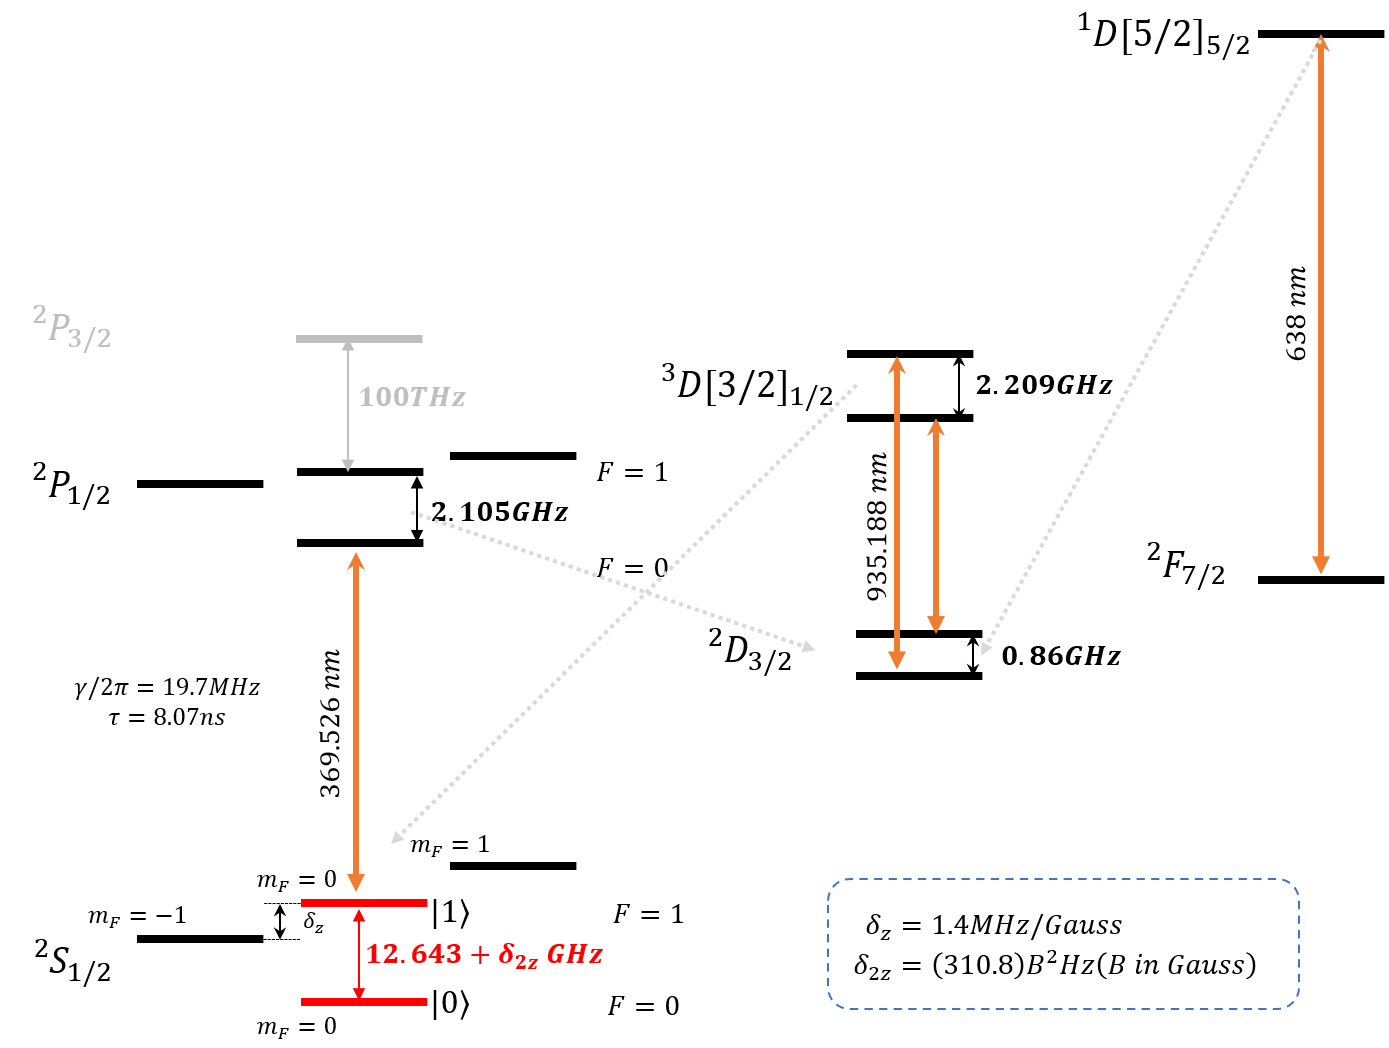
\includegraphics[width=1.0\linewidth]{energy_structure}
\end{figure}

通过在阱外向阱中离子施加的约$6$高斯的静磁场会使离子产生约$11$Hz的二阶\emph{Zeeman}能级劈裂。从$\ket{1}$态向$^2P_{1/2}$能级跃迁回路的驱动波长在$369.526$nm附近,这个波段的激光有成熟的商业激光系统供应,同时对光纤传输也很友好。略有遗憾的是这个$\ket{1}^2P_{1/2}$跃迁回路并不是完全闭合的,因为存在从$^2P_{1/2}$到$^2D_{3/2}$的微弱态泄露,分支比约为$0.5$\%\cite[]{Olmschenk_Younge_Moehring_Matsukevich_Maunz_Monroe_2007}。不过这个可以通过使用一个带$3.07$GHz边带的$935$nm波长的激光来将泄露的态再回泵浦到整个回路中。另外,背景撞击可能导致离子跑到$^2F_{7/2}$使离子“熄灭”,这个可以通过一个$638$nm波长的激光器来克服,重新将离子“点亮”。值得注意的是,这个任务除了$638$nm波长的激光器可以完成外,$760$nm\cite[]{Huntemann_Okhapkin_Lipphardt_Weyers_Tamm_Peik_2012}、$355$nm\cite[]{Senko_2014}。另外,由于从$2^F_{7/2}$到$3^F[1/2]_{3/2}$的跃迁大部分共振在$375.856$nm波长上,因此$375$nm波长的激光也可以完成。

\section[镱离子的电离和囚禁]{镱离子的电离和囚禁}
为了能够研究离子的特性我们首先需要将离子电离并稳定地囚禁住。离子的囚禁采用的是如第\ref{section:ion_classical_motion}节中介绍的动态囚禁的方式,离子的电离一般是通过激光电离的方式实现的。对于$Yb^+$离子来说,电离的方式是采用的是\emph{两步电离法(two-step ionization)}\cite[]{Olmschenk_Younge_Moehring_Matsukevich_Maunz_Monroe_2007},这种方法可以避免紫外激光的使用。
首先,我们使用$398.991$nm波长的激光将镱原子重$^1S_0$能级激发到$^1P_1$能级;然后再使用一个低于$394.088$nm波长的激光将最外层电子激发到连续态区域中去,比如通常采用的$369.526$nm波长激光,或者$355$nm波长、$375$nm波长。在实践中,镱原子一般填充在原子炉中并被放置在真空室中。需要激发时就通过施加恒定电流加热原子,使原子从烤箱中热喷射出来的,其中会有一小部分穿过离子阱的中心。$398.911$nm和$369.525$nm波长的激光束在离子阱中心与原子炉中喷射出的原子重叠。于是,该区域的原子就可以被电离,并在高效冷却后被离子阱动态囚禁。由于同位素位移,我们可以通过微调$398.911$nm激光的波长来选择性地电离镱离子不同的同位素。为了抑制多普勒频移的影响,激光器的路径最好垂直于原子流。

\begin{figure}
    \centering
    \caption[刀片阱示意图]{刀片阱示意图\label{fig:trap_blads}}
    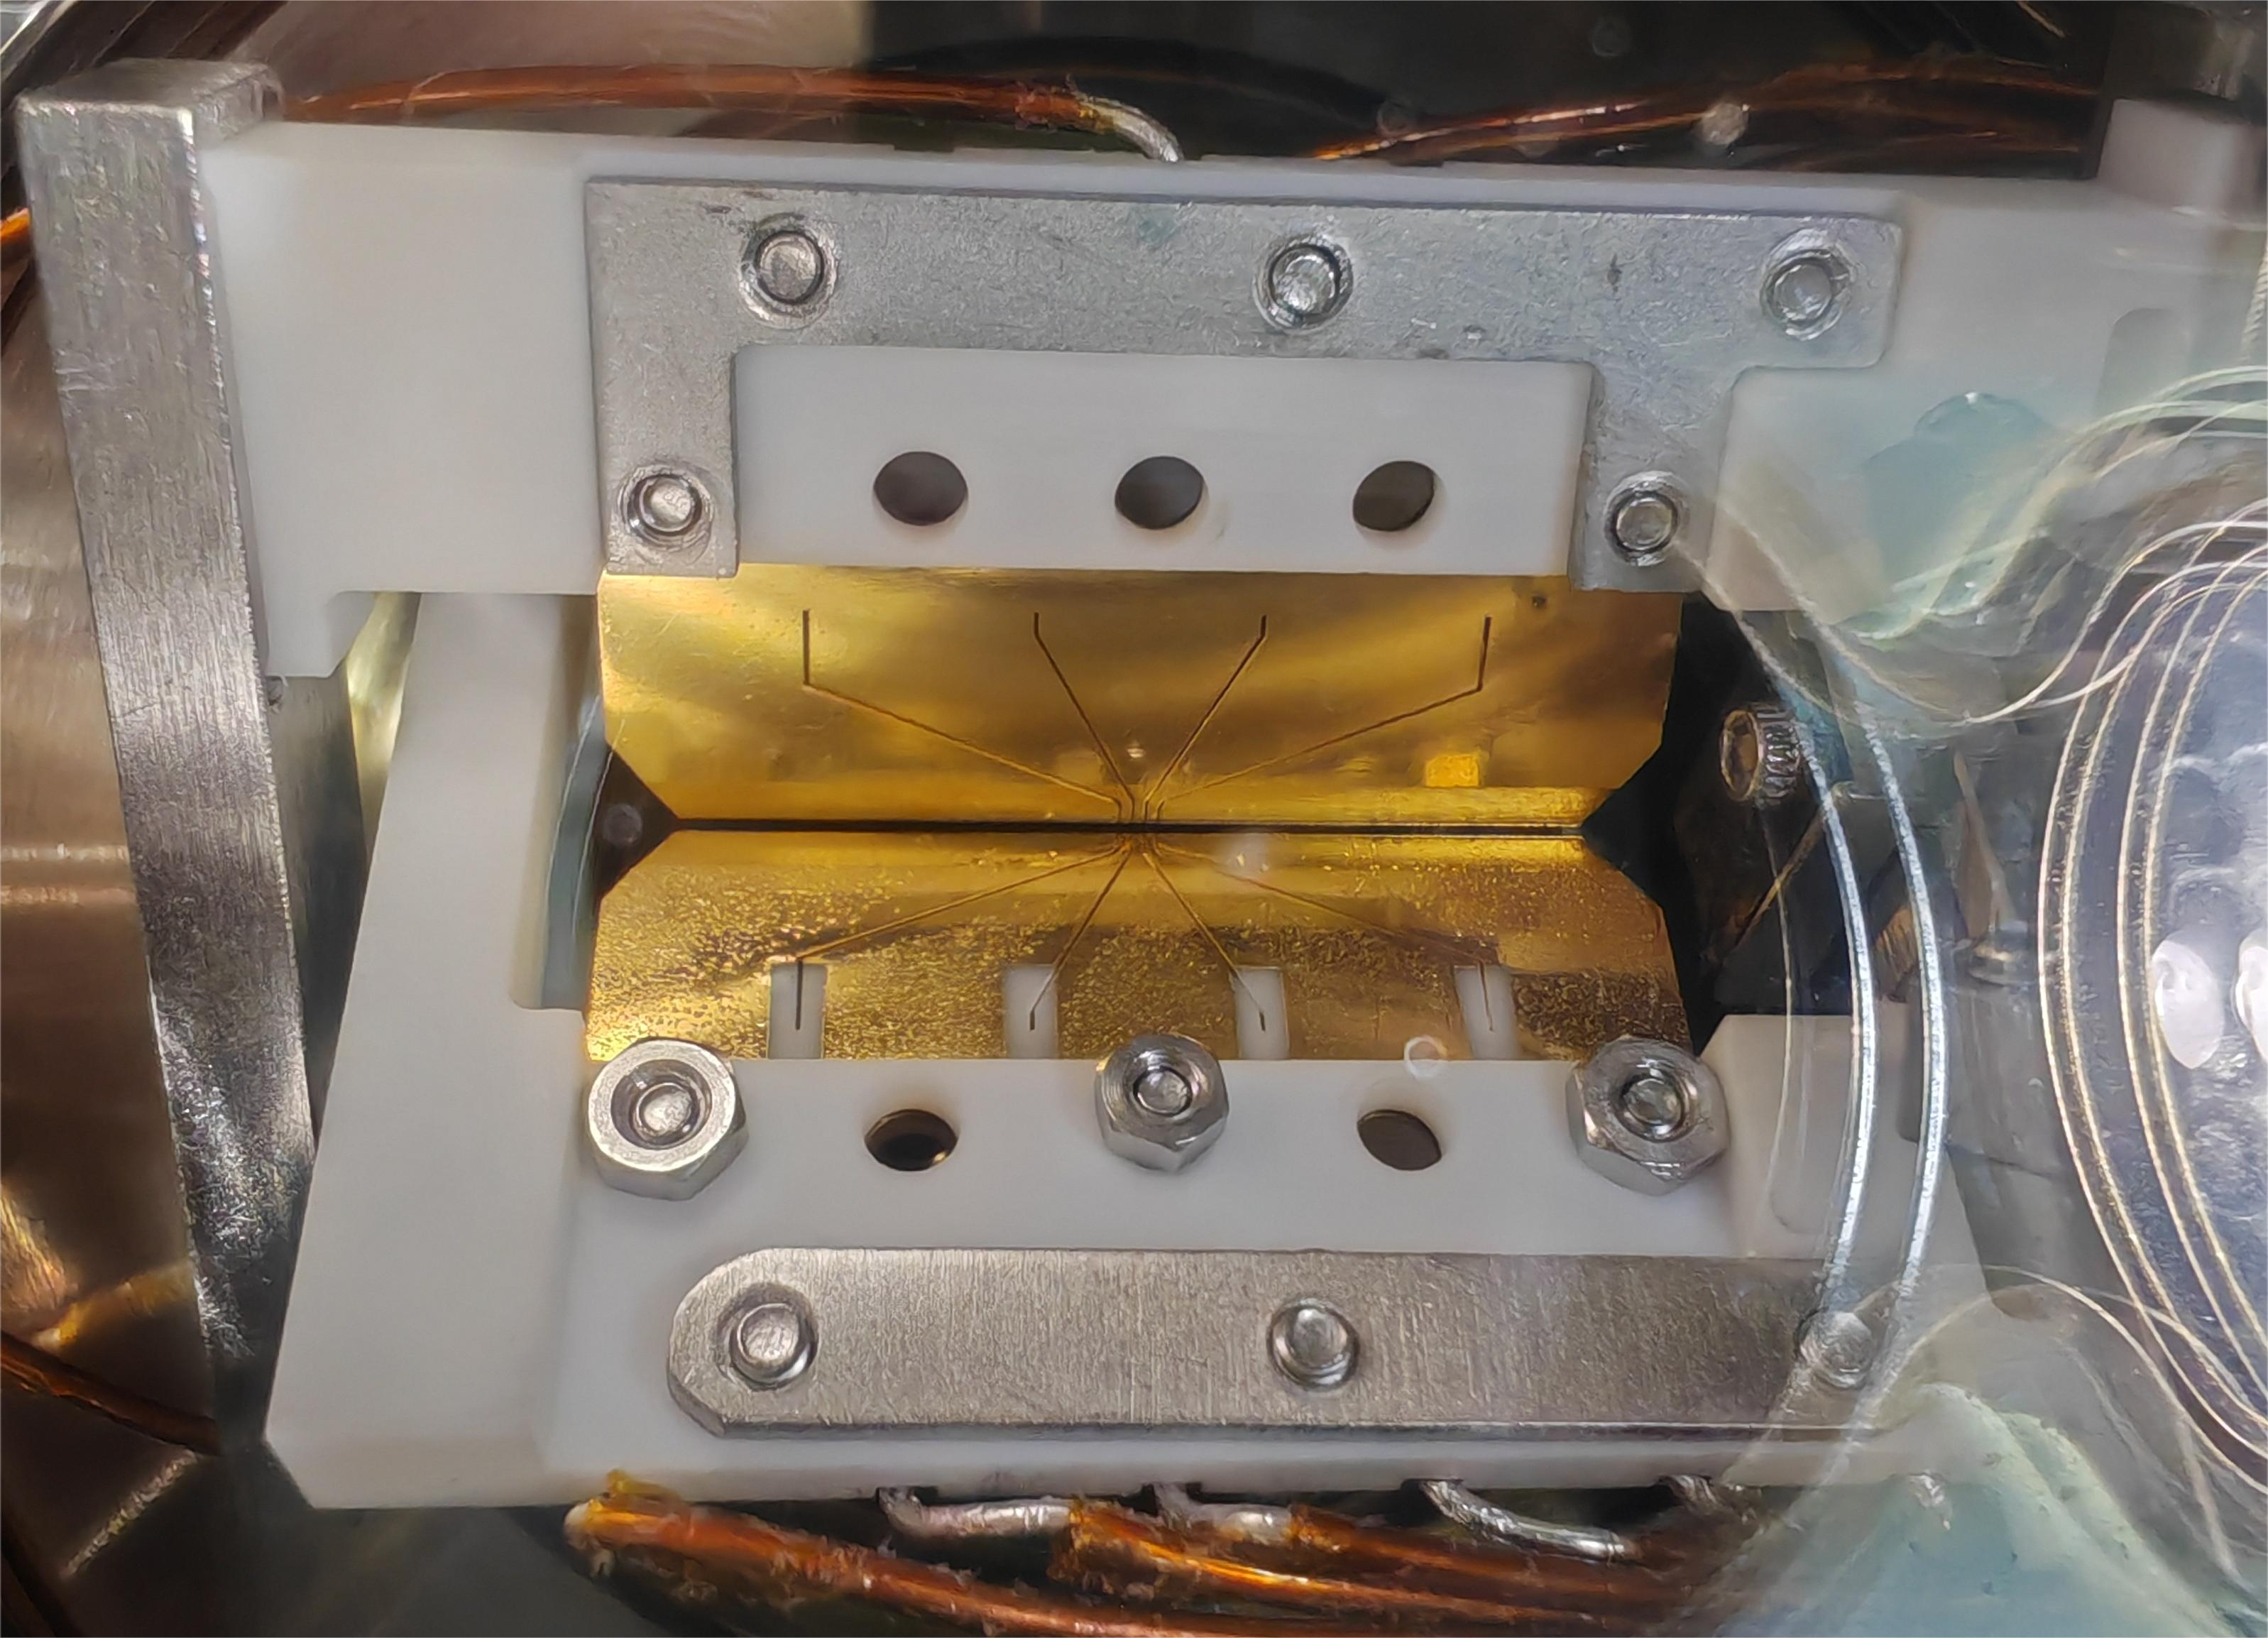
\includegraphics[width=1.0\linewidth]{trap_blads}
\end{figure}

如第\ref{section:ion_classical_motion}节中给介绍的,由\emph{Earnshaw's theorem}\cite[]{Earnshaw}我们知道离子没有办法被静态地囚禁在三维空间中,好在我们仍然可以动态地将离子囚禁。实际实验中囚禁离子的离子阱如\ref{fig:trap_blads}图所示,这中类型的离子阱一般被称为刀片阱。它会产生如下形式的赝势$\Phi_p$:
\begin{align}
    \Phi_p=\frac{eV^2}{4MR^4\Omega_{rf}^2}\sum_{m}^{}\alpha_m^2r_m^2
\end{align}

其中$V$,$R$,$M$分别是RF电压、电极到阱中心的距离和离子的质量。$\Omega_{rf}$是RF的频率,$\alpha_m$是$r_m$方向的系数。
这个电势的结果是在所有方向上都有正的系数 ($\alpha_m^2>0$),直观地揭示了囚禁带电离子的能力。同时还可以从中得到有效的阱频率$\nu_m=eV\alpha_m/\sqrt{2}MR^2\Omega_{rf}$。

\section[镱离子的激光冷却]{镱离子的激光冷却\label{section:yb_laser_cooling}}
从原子炉中喷出的原子是十分“热”的(标准大气压下原子的平均融化温度高达$824 ^o C$),由麦克斯韦运动分布可知它们的速度能达到超过一百米每秒。如此热的电子很容易从离子阱的囚禁电势中逃脱,很难被囚禁更不用说惊醒什么别的操作了。因此,我们需要某种冷却手段来给离子“降温”。

\begin{figure}
    \centering
    \caption[激光施加到离子的多普勒效应示意图]{激光施加到离子的多普勒效应示意图\label{fig:doppler_cooling_scattering}}
    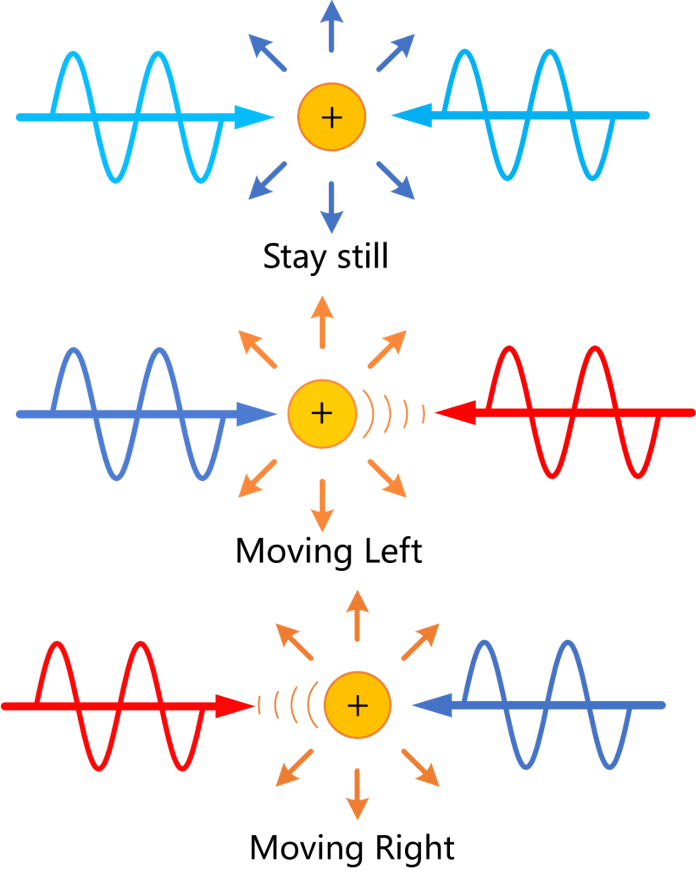
\includegraphics[width=1.0\linewidth]{doppler_cooling_scattering}
\end{figure}
离子可以使用红色失谐的反向传播激光束进行激光冷却,这被称为多普勒冷却\cite[]{Hänsch_Schawlow_1975}。如图\ref{fig:doppler_cooling_scattering}所示,当离子与激光反向运动时,吸收一个光子离子将减少$\hbar \vec{k}$的动量;当离子与光同向运动时,吸收一个光子离子将增加$\hbar \vec{k}$的动量。随后离子将通过受激辐射的形式随机散射$\hbar \vec{k}$的动量,这个随机散射过程的平均结果是动量变化为$0$。

\begin{figure}
    \centering
    \caption[多普勒冷却示意图]{多普勒冷却示意图\label{fig:doppler_cooling}}
    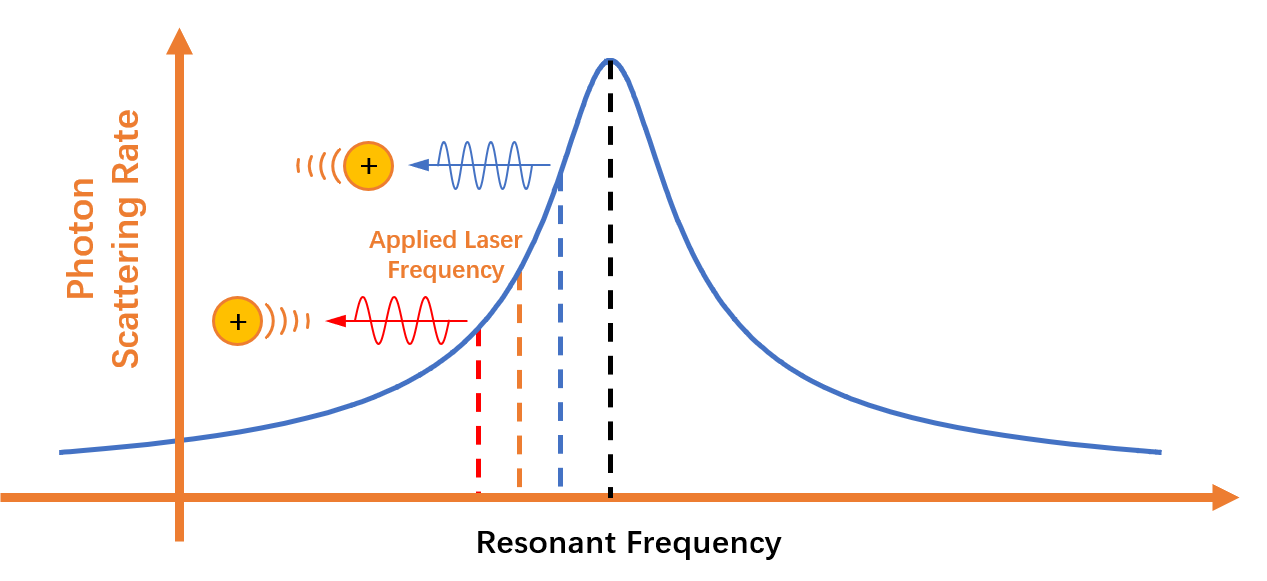
\includegraphics[width=1.0\linewidth]{doppler_cooling}
\end{figure}
如图\ref{fig:doppler_cooling}所示,由于多普勒效应,在离子局部坐标系下看入射激光的波长会产生$-\vec{k}\cdot\vec{v}$的频移。因此如果施加红是失谐的激光,那么与激光方向相反的离子将比与激光方向相同的离子吸收更多的光子;另一方面,对打的激光会抵消激光本身对离子的加速效应,最终离子会失去较多的动量,被激光“冷却”下来。

对$Yb^+$离子来说,在这个过程中跃迁$2^S_{1/2}\ket{F=1}\to ^2P_{1/2\ket{F=0}}$和$2^S_{1/2}\ket{F=0}\to ^2P_{1/2\ket{F=1}}$同时被驱动以覆盖离子的所有超精细能级,避免离子陷入暗态(变黑)。

此外,冷却激光的所有偏振都施加上去来提高冷却效率,相关跃迁回路和离子散射图如图\ref{fig:doppler_cooling_level}所示。
\begin{figure}
    \centering
    \caption[离子冷却跃迁回路示意图]{离子冷却跃迁回路示意图\label{fig:doppler_cooling_level}}
    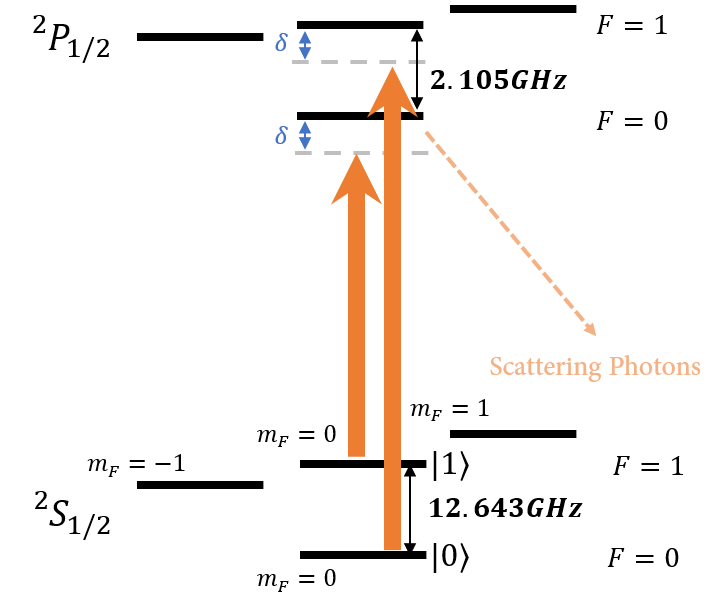
\includegraphics[width=1.0\linewidth]{doppler_cooling_level}
\end{figure}

\section[镱离子的态初始化]{镱离子的态初始化\label{section:yb_state_init}}

几乎任何量子计算或模拟任务都以确定性的纯状态开始。获得这个起点的过程称为\emph{态初始化(State Initialization)},这是通过囚禁离子平台中的光泵浦过程实现的。

\begin{figure}
    \centering
    \caption[离子态初始化示意图]{离子态初始化示意图\label{fig:initialization}}
    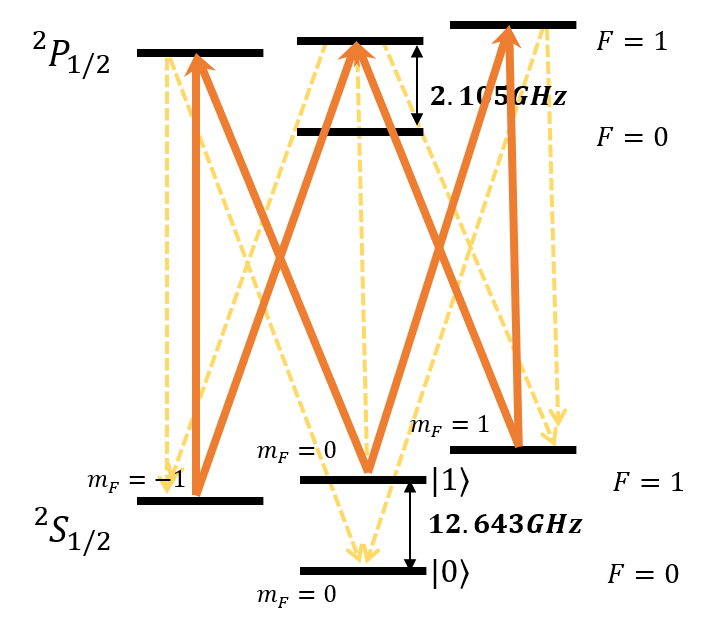
\includegraphics[width=1.0\linewidth]{initialization}
\end{figure}

如图\ref{fig:initialization}所示,在初始化过程中从$^2S_{1/2}\ket{F=1}$到$^2P_{1/2}\ket{F=1}$的跃迁被驱动。离子的状态很有可能衰减到$\ket{0}$状态,因此由于$12.6$GHz的失谐,处于$\ket{0}$态的离子不会参与进一步的激发。对于单个离子,这一过程在$5$μs内就可以以非常高的初始化保真度完成。这篇\cite[]{Harty_Allcock_Ballance_Guidoni_Janacek_Linke_Stacey_Lucas_2014}文献展示了状态初始化的误差小于可以$10^{−4}$

\section[镱离子的态探测]{镱离子的态探测\label{section:yb_state_detection}}
在经过各种中间操控后,量子计算的结果需要被读出,这一过程通过离子的态测量实现。如图\ref{fig:detection}所示,通常采用状态相关的荧光检测技术进行高保真读出\cite[]{Blinov_Leibfried_Monroe_Wineland_2004}。在这个过程中使用的是$^2S_{1/2}\ket{F=0}$到$^2P_{1/2}\ket{F=1}$之间的跃迁($^2S_{1/2}\ket{F=0}$到$^2P_{1/2}\ket{F=0}$之间的跃迁是偶极禁止跃迁的)。因此,我们可以通过数收集散射光子的数量的多少来区分投影状态。
\begin{figure}
    \centering
    \caption[离子态测量示意图]{离子态测量示意图\label{fig:detection}}
    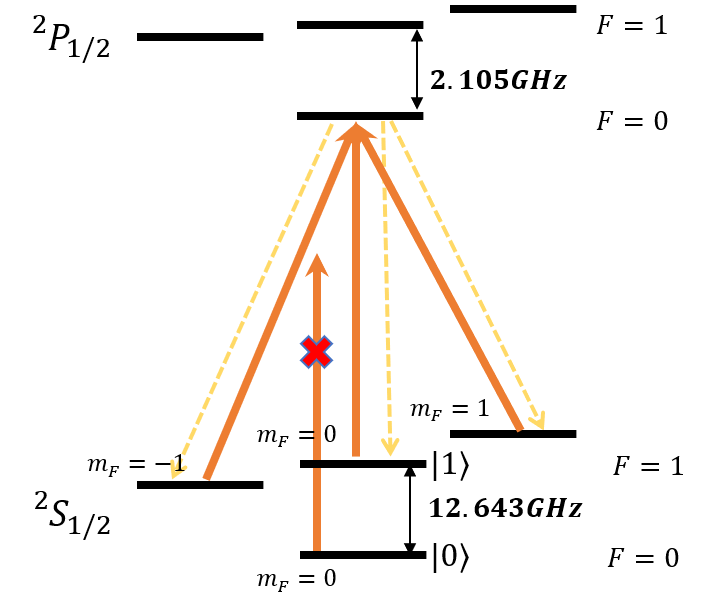
\includegraphics[width=1.0\linewidth]{detection}
\end{figure}

态测量过程得到的离子影像可以用\emph{电子倍增电荷耦合器件(Electron-multiplying charge-coupled device, EMCCD)}或者\emph{光电倍增管(Photomultiplier Tube, PMT)}通过两步成像来显示,如图\ref{fig:two_step_imaging}所示。
对于单个离子,为了量化量子比特状态检测的保真度,我们可以将量子比特准备为$\ket{0}$状态或$\ket{1}$状态,然后应用持续$40$μs的探测激光束同时计数收集到的光子。每个状态的序列通常重复$2000$次以获得统计分布。

\begin{figure}
    \centering
    \caption[两步成像系统]{两步成像系统\label{fig:two_step_imaging}}
    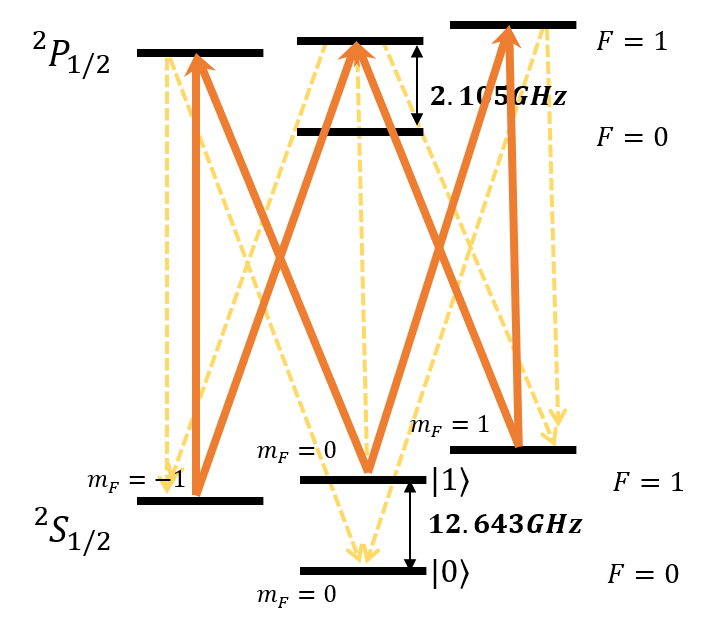
\includegraphics[width=1.0\linewidth]{two_step_imaging}
\end{figure}

以我们目前系统为例,入射光子数量的统计数据几乎遵循泊松分布,$\ket{0}$和$\ket{1}$状态的平均光子分别为$0.05$和$9.58$。分离良好的分布使我们能够将投影状态与固定阈值区分开来。对于单次检测,如果收集到的光子数大于1,则我们将投影状态分类为$\ket{1}$状态,否则投影状态被视为$\ket{0}$状态。

\section[镱离子的态操控]{镱离子的态操控\label{section:yb_state_manipulation}}
量子门可以通过微波\cite[]{Olmschenk_Younge_Moehring_Matsukevich_Maunz_Monroe_2007}或脉冲激光\cite[]{Lee_2005}实现。微波对离子的态操控实现简单,但是由于所用微波的长波太长,使用微波技术方案往往仅限于单比特门;激光操控离子有诸多优点,尤其是在大规模的集成和寻址方面。接下来的小节将具体介绍这两类离子比特门操控方式。
\subsection[微波操控镱离子]{微波操控镱离子}
在本小节中,我将简要介绍微波操控的离子量子门,以帮助建立离子态操控的一般方式。
在微波场下的离子哈密顿量为(保持$\hbar=1$):
\begin{align}
    \hat{H}=\frac{\omega_q}{2}\hat{\sigma}_z + \Omega\cos\left(\vec{k}\cdot\vec{r}-\omega t + \phi\right)\hat{\sigma}_x
\end{align}

第一项是简化的离子比特二能级系统的希尔伯特空间,二能级系统的能量差为$\omega_q$;第二项是磁偶极跃迁的导出项,其中磁场的振动频率为$\omega$,初始相位为$\phi$;$\Omega$是代表耦合强度的拉比频率;当$\omega\approx 12.6$GHz时有$\vec{k}\approx3\times ^{-4}um^{-1}$,所以空间项$\vec{k}\cdot \vec{r}$相对比较小,可以被忽略。通过一个重映射变换$\hat{H}_I=e^{iH_0t}(\hat{H}-\hat{H}_0)e^{-iH_0t}$,其中$\hat{H}_0=\omega\hat{\sigma}_z/2$,可以将自由空间哈密顿量转化到相互作用表象\textcolor{red}{(dressed-state)}下:
\begin{align}
    \hat{H}_I&=e^{iH_0t}(\hat{H}-\hat{H}_0)e^{-iH_0t}\\
    &=-\frac{\mu}{2}\hat{\sigma}_z+\frac{\Omega}{2}\left(\hat{\sigma}_+e^{i\omega t}+\hat{\sigma}_-e^{-i\omega t}\right)\left(e^{i(\omega t-\phi)}+e^{-i(\omega t-\phi)}\right)\\
    &\approx -\frac{\mu}{2}\hat{\sigma}_z+\Omega(\hat{\sigma}_+e^{i\phi}+\hat{\sigma}_-e^{-i\phi})\\
    &=-\frac{\mu}{2}\hat{\sigma}_z+\frac{\Omega\cos{\phi}}{2}\hat{\sigma}_x+\frac{\Omega\sin{\phi}}{2}\hat{\sigma}_y
\end{align}

其中$\mu=\omega=\omega_q$是量子比特和单微波光子之间的能量差。在$\approx$这步,我们采用了在第\ref{section:total_hamiltonian}节中介绍过的\emph{旋波近似},将含$2\omega$的快速振动项忽略掉了。相互作用表象\textcolor{red}{(dressed-state)}的优点在于最终的哈密顿量是不含时的,这样各个泡利矩阵的成分的概率幅就完全由施加的微波场决定了。

对于一个给定的状态$\ket{\Psi(0)}=c_0(0)\ket{0}+c_1(0)\ket{1}$,其中$|c_0(0)|^2+|c_1(0)|^2=1$,它的时间演化由演化算符$U(t)$决定:
\begin{align}
    \ket{\Psi(t)}=U(t)\ket{\Psi(0)}=\exp(-iH_It)\ket{\Psi(0)}
\end{align}

如果给定$\ket{\Psi(0)}=\ket{0}$,那么可以解析地写出这个态的演化后的概率幅:
\begin{align}
    c_1(t)=-i\frac{\Omega}{\Omega_{eff}}e^{i\phi}\sin{\frac{\Omega_{eff}t}{2}},\\
    c_0(t)=\cos{\frac{\Omega_{eff}t}{2}}-i\frac{\mu}{\Omega_{eff}}\sin{\frac{\Omega_{eff}t}{2}}
\end{align}

其中$\Omega_{eff}=\sqrt{\Omega^2+\mu^2}$是有效拉比频率[77]。$\ket{1}$态的概率$p_1(t)=|c_1(t)|^2$在时间$t=\pi/\Omega_{eff}$时取得最大值,最大值为$\Omega^2/(\Omega^2+\mu^2)$。不同失谐$\mu$情况下的拉比振荡如图所示。

\begin{figure}
    \centering
    \caption[不同失谐$\mu$情况下的拉比振荡]{不同失谐$\mu$情况下的拉比振荡\cite[]{Lu_2019}}
    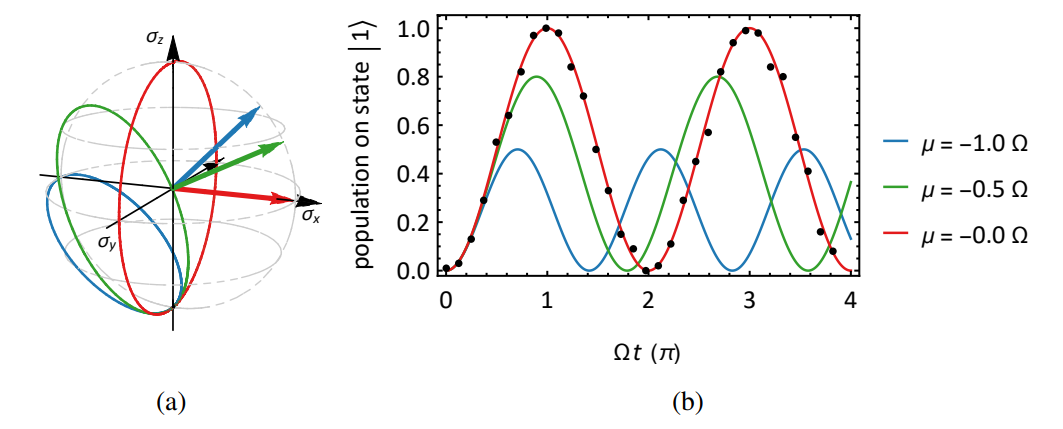
\includegraphics[width=1.0\linewidth]{rabi_oscillations}
\end{figure}

碎玉量子计算的实现,我们总是使$\mu\approx0$以实现任意单比特的旋转操控:
\begin{align}
    R_\phi(\theta)=U\left(\frac{\theta}{\Omega},P\phi\right)=\exp[-i\frac{\theta}{2}\sigma_\phi]
\end{align}

其中$\sigma_\phi=\sigma_x\cos{\phi}+\sigma_y\sin{\phi}$。对于初始状态,在$\theta=\pi$或者说是$t=\pi/\Omega$时,初始态的概率可以完全转移到二能级系统的另一个态上。这种$R_\phi(\theta)$旋转操作被称为沿着$\phi$轴的态旋转操控,$R_\phi(\pi)$被称为$\pi$翻转,它的作用类似之前在第\ref{section:reversible_gates}节中介绍过的经典的NOT门。除此之外,还有一种重要的旋转操作$R_\phi(\pi/2)$,它常被称为$\pi/2$翻转,可以用来制备十分有用的叠加态$(\ket{0}+e^{-i\phi}\ket{1})/\sqrt{2}$。








\subsection[连续激光操控镱离子]{连续激光操控镱离子}

\subsection[脉冲激光操控镱离子]{脉冲激光操控镱离子}

\section[Mølmer-Sørensen 门]{Mølmer-Sørensen 门}